\documentclass[12pt]{article}
\usepackage{geometry}
\geometry{a4paper}
\usepackage[utf8]{inputenc}
\usepackage{graphicx}
\usepackage{hyperref}
\usepackage{amsmath}
\usepackage{amsfonts}
\usepackage{amssymb}
\usepackage{listings}
\usepackage{float}

\lstset{
    basicstyle=\ttfamily\small, % Set the size of the code font
    breaklines=true, % Enables line breaking
}
\usepackage{color} % Required for custom colors
\usepackage{fancybox} % Required for box settings around the code
\usepackage{xcolor} % More advanced color handling

\definecolor{keywordcolor}{rgb}{0,0,1} % Blue for keywords
\definecolor{capitalletter}{rgb}{2.5,0,0} % Dark red for capital letters

% Custom language style for Cypher
\lstdefinelanguage{Cypher}{
    morekeywords={MATCH, CREATE, RETURN, MERGE, LOAD, CSV, WITH, HEADERS, FROM, AS, WHERE},
    sensitive=false,
    morecomment=[l]{//},
    morestring=[b]",
    keywordstyle=\color{keywordcolor}\bfseries,
    identifierstyle=\color{capitalletter},
    stringstyle=\color{black},
    commentstyle=\color{purple}
}

\lstset{
    language=Cypher,
    frame=single,
    extendedchars=true,
    basicstyle=\ttfamily\small,
    showstringspaces=false,
    showspaces=false,
    numbers=left,
    numberstyle=\small,
    numbersep=9pt,
    tabsize=2,
    breaklines=true,
    showtabs=false,
    captionpos=b
}



\title{\textbf{KSE30 Companies Network Analysis}}
\author{CS-343: Graph Data Science \\Habib University \\By: Abdullah Junejo (07154)  Alizain Merchant (07565) }
\date{Final Report\\ - \\ Date: \today}

\begin{document}

\maketitle

\section{Introduction}
%This section provides an overview of the project's scope, objectives, and the significance of using graph databases in managing governmental data.
In this project, we explore the intricate and ever-evolving landscape of the Karachi Stock Exchange 30 (KSE30) Index, which represents the top 30 corporations in Pakistan by market capitalization and liquidity. Our goal is to employ graph database technology to dissect and elucidate the complex web of relationships and interdependencies among these premier entities. Utilizing graph databases enables us to represent and probe these relationships with unmatched intuitiveness and efficiency. Specifically, by mapping the KSE30 companies and their principal executives and board members as nodes within a graph database, we seek to shed light on the influence of these individuals within the market, explore their network connections, and analyze overall market trends. For this purpose, we will utilize Neo4j, gathering our data directly from the Pakistan Stock Exchange through the PSX Data Portal (https://dps.psx.com.pk/).
\section{Data Collection}
The Data was manually collected by going into the PSX Data Portal and then KSE30 where we saw different market performers. Upon clicking the company and noting down its information one by one, we were able to put together a .csv file for this (Attached). This task can be furthered on KSE100 as well after successful demonstration of this miniature project.
\section{Data Modelling/Import}
Here is our initial Graph Model that we will use. Hoever, his may very well be improvised upon in the future! \\
\begin{figure}[htbp]
    \centering
    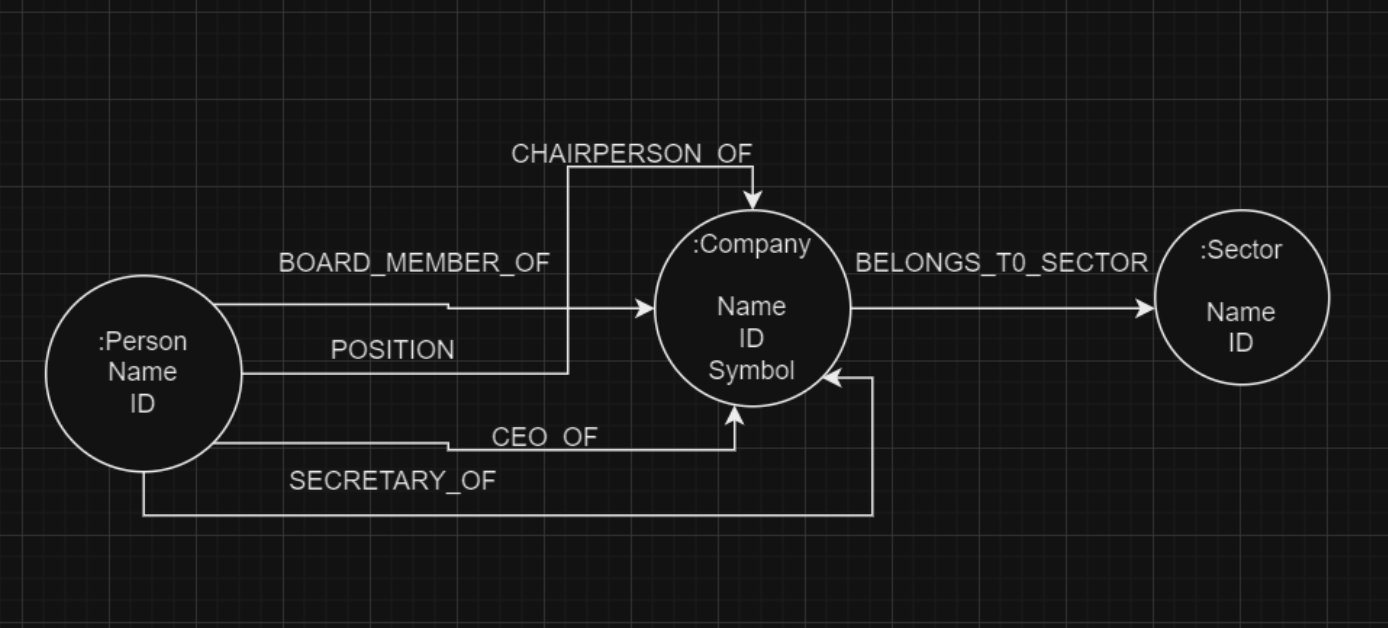
\includegraphics[width=0.9\textwidth]{Initial_Model.png} % Replace example-image with the filename of your image
    \caption{Initial Model}
  \end{figure}
\\
After Creating Project, Installing Graph Data Science/APOC Libraries, dropping the file in import folder, we worked on this script and used it to import data our csv file according to our afforementioned model.
\begin{lstlisting}[frame=single]
    LOAD CSV WITH HEADERS FROM 'file:///KSE_30_Formatted.csv' AS row
    WITH row
    WHERE row.Board of Directors IS NOT NULL AND TRIM(row.Board of Directors) <> ""
    UNWIND SPLIT(row.Board of Directors, ";") AS directorDetails
    WITH row, TRIM(directorDetails) AS directorDetails
    WHERE directorDetails <> ""
    WITH row, 
         TRIM(SPLIT(directorDetails, "(")[0]) AS DirName, 
         TRIM(SPLIT(SPLIT(directorDetails, "(")[1], ")")[0]) AS position
    WHERE row.Year IS NOT NULL AND TRIM(row.Year) <> ""
      AND row.Company Sector IS NOT NULL AND TRIM(row.Company Sector) <> ""
      AND row.Secretary IS NOT NULL AND TRIM(row.Secretary) <> ""
      AND row.Chairperson IS NOT NULL AND TRIM(row.Chairperson) <> ""
      AND row.Company Symbol IS NOT NULL AND TRIM(row.Company Symbol) <> ""
      AND row.Company Name IS NOT NULL AND TRIM(row.Company Name) <> ""
      AND row.Company CEO IS NOT NULL AND TRIM(row.Company CEO) <> ""
      AND position IS NOT NULL AND TRIM(position) <> ""
    
    MERGE (company:Company {name: row.Company Name, symbol: row.Company Symbol})
    MERGE (sector:Sector {name: row.Company Sector})
    MERGE (chairperson:Person {name: row.Chairperson})
    MERGE (secretary:Person {name: row.Secretary})
    MERGE (ceo:Person {name: row.Company CEO})
    
    WITH company, sector, chairperson, secretary, ceo, DirName, position
    MERGE (director:Person {name: DirName})
    MERGE (director)-[:BOARD_MEMBER_OF {position: position}]->(company)
    MERGE (company)-[:CHAIRPERSON_OF]->(chairperson)
    MERGE (company)-[:SECRETARY_OF]->(secretary)
    MERGE (company)-[:CEO_OF]->(ceo)
    MERGE (company)-[:BELONGS_TO_SECTOR]->(sector);
\end{lstlisting}

After this, it became aparent that there were multiple edges of "Board Member" from the same Person Node to the Same Company Node but having different edge property called position. So we decided to merge them so that future queries are easier and performance is not compromised.  The property of position was also in a way merged. Different positions were seperated by a backslash.
\begin{lstlisting}[frame=single]
//Step 1: Match and collect positions for each director-company pair
MATCH (director:Person)-[r:BOARD_MEMBER_OF]->(company:Company)
WITH director, company, COLLECT(DISTINCT r.position) AS positions, COLLECT(r) AS rels

//Step 2: Delete the existing relationships
FOREACH (rel in rels | DELETE rel)

//Step 3: Create a new single relationship with all positions combined
WITH director, company, REDUCE(s = "", position IN positions | s + (CASE WHEN s = "" THEN "" ELSE "\\" END) + position) AS combinedPositions
MERGE (director)-[newRel:BOARD_MEMBER_OF]->(company)
SET newRel.positions = combinedPositions
\end{lstlisting}
This essentially merged Multiple Board of Director edges into one if they are related to the same company.
\section{Graph Statistics}
This initial statistic provides a snapshot of the various sectors represented in the KSE30 index, the total number of companies, and detailed counts of key executive roles across all companies. This fundamental data lays the groundwork for deeper analyses, offering a clear view of the breadth and scope of leadership within these influential companies. 
\begin{lstlisting}[frame=single]
    //Statistics 1:
MATCH (sector:Sector)
WITH COLLECT(sector.name) AS Sector Names

MATCH (company:Company)
WITH Sector Names, COUNT(company) AS Total Number of Companies

MATCH (director:Person)-[:BOARD_MEMBER_OF]->(company)
WITH Sector Names, Total Number of Companies, COUNT(DISTINCT director) AS Total Number of Board Members

MATCH (chairperson:Person)<-[:CHAIRPERSON_OF]-(company)
WITH Sector Names, Total Number of Companies, Total Number of Board Members, COUNT(DISTINCT chairperson) AS Total Number of Chairpersons

MATCH (ceo:Person)<-[:CEO_OF]-(company)
WITH Sector Names, Total Number of Companies, Total Number of Board Members, Total Number of Chairpersons, COUNT(DISTINCT ceo) AS Total Number of CEOs

MATCH (secretary:Person)<-[:SECRETARY_OF]-(company)
RETURN Sector Names, Total Number of Companies, Total Number of Board Members, Total Number of Chairpersons, Total Number of CEOs, COUNT(DISTINCT secretary) AS Total Number of Secretaries

\end{lstlisting}
This second analysis reveals directors who hold positions across multiple companies (Highest 2 as of now), which could give a general idea about their influence across corporations and potential conflicts of interest. Next query is about tracking chairpersons who currently oversee multiple companies ($\exists$ 1 such chairperson as of now) further sheds light on the leadership dynamics. The third query tries to find the company that sits at the center of the most extensive connections, either through direct executive roles such as secretary, chairperson, CEO or through other types of affiliative relationships such as Board Member. Such a company typically acts as a central node within the network which we hope to unravel and confirm in our future explorations.
Next we try to Highlight the sector that includes the most companies within the KSE30 offers insights into which part of the economy is most saturated. This information is crucial for steering investment strategies, creating economic policies (regarding subsidy/taxation), and conducting market analysis, as it reflects the sector's economic significance and its potential for expansion or risk.

\begin{lstlisting}[frame=single]
    //Statistics 2: 
    // Collect data for board members belonging to multiple companies
    MATCH (director:Person)-[:BOARD_MEMBER_OF]->(company:Company)
    WITH director, COUNT(DISTINCT company) AS Number of Companies
    WHERE Number of Companies > 1
    WITH COLLECT(director.name) AS Multi Company Board Members
    
    // Collect data for chairpersons of multiple companies
    MATCH (chairperson:Person)<-[:CHAIRPERSON_OF]-(company:Company)
    WITH chairperson, COUNT(DISTINCT company) AS Number of Companies, Multi Company Board Members
    WHERE Number of Companies > 1
    WITH COLLECT(chairperson.name) AS Multi Company Chairpersons, Multi Company Board Members
    
    // Identify the company with the most affiliations
    MATCH (person:Person)-[r]->(company:Company)
    WITH company, COUNT(DISTINCT person) AS Number of Affiliates, Multi Company Board Members, Multi Company Chairpersons
    ORDER BY Number of Affiliates DESC
    WITH COLLECT({companyName: company.name, numAffiliates: Number of Affiliates})[0] AS Company With Most Affiliates, Multi Company Board Members, Multi Company Chairpersons
    
    // Sector with the most companies
    MATCH (company:Company)-[:BELONGS_TO_SECTOR]->(sector:Sector)
    WITH sector, COUNT(DISTINCT company) AS Number of Companies, Company With Most Affiliates, Multi Company Board Members, Multi Company Chairpersons
    RETURN sector.name AS Sector with Most Companies, Number of Companies, 
           Company With Most Affiliates.companyName AS Company with Most Affiliations, 
           Company With Most Affiliates.numAffiliates AS Number of Affiliated Persons,
           Multi Company Board Members, 
           Multi Company Chairpersons
    ORDER BY Number of Companies DESC
    LIMIT 1
\end{lstlisting}

These statistics, derived from targeted Cypher queries, do more than just quantify the interconnections within the KSE30. They also provide a deeper qualitative understanding of corporate governance and sectoral prominence, laying a robust foundation for further analysis such as predictive modeling and trend examination. This enriched insight is instrumental in comprehensively understanding the dynamics that shape Pakistan's economic forefront.


\section{Creating Further Data}
Our data was mostly homogenous clusters of companies and their executives. Only few Board Members were part of 2 companies and only 1 chairperson. This shows that for our future analytics, it could be difficult to find a person to person shortest path. This is why we introduce government as stakeholders. It is a natural and well founded assumption that companies belonging to a sector will be regulated by the relavant government agencies. The company executives will have the meetings with such ministries and would be able to connect with their head, The minister. This could provide us a path to other clusters that was otherwise isolated. The Data was manually collected from Wikipedia and verified from various other official government web sources.
\begin{lstlisting}[frame=single]
    //Creation of Ministries
    CREATE (energy:Ministry {name: "Ministry of Energy"}),(sbp:Ministry {name: "State Bank of Pakistan"}),(itTelecom:Ministry {name: "Ministry of Information Technology and Telecommunication"}),(scienceTech:Ministry {name: "Ministry of Science and Technology"}),(foodSecurity:Ministry {name: "Ministry of National Food Security and Research"}),
    (industries:Ministry {name: "Ministry of Industries and Production"}),
    (commerceTextile:Ministry {name: "Ministry of Commerce and Textile Industry"}),
    (health:Ministry {name: "Ministry of National Health Services, Regulations and Coordination"});

    //Link Ministries to Sectors
    MATCH (ministry:Ministry), (sector:Sector)
    WHERE (ministry.name = "Ministry of Energy" AND sector.name IN ["Refinery", "Power Generation & Distribution", "Oil & Gas Marketing Companies", "Oil & Gas Exploration Companies"]) OR
          (ministry.name = "Ministry of Information Technology and Telecommunication" AND sector.name = "Technology & Communication") OR
          (ministry.name = "Ministry of Science and Technology" AND sector.name = "Chemical") OR
          (ministry.name = "Ministry of National Food Security and Research" AND sector.name = "Food & Personal Care Products") OR
          (ministry.name = "State Bank of Pakistan" AND sector.name = "Commercial Banks") OR
          (ministry.name = "Ministry of Industries and Production" AND sector.name IN ["Cement", "Cable & Electrical Goods"]) OR
          (ministry.name = "Ministry of Commerce and Textile Industry" AND sector.name = "Textile Spinning") OR
          (ministry.name = "Ministry of National Health Services, Regulations and Coordination" AND sector.name = "Pharmaceuticals")
    MERGE (sector)-[:REGULATED_BY]->(ministry);

    //Creation of Minister Nodes and Linking to Ministries with Positions

    //Minister of Energy
    CREATE (musadikMalik:Person {name: "Musadik Masood Malik", position: "Minister"})
    WITH musadikMalik
    MATCH (ministryEnergy:Ministry {name: "Ministry of Energy"})
    MERGE (musadikMalik)-[:HEADS]->(ministryEnergy)
    
    //Minister of Information Technology and Telecommunication
    CREATE (shazaFatima:Person {name: "Shaza Fatima Khawaja", position: "Minister"})
    WITH shazaFatima
    MATCH (ministryIT:Ministry {name: "Ministry of Information Technology and Telecommunication"})
    MERGE (shazaFatima)-[:HEADS]->(ministryIT)
    
    //Minister of Science and Technology
    CREATE (khalidSiddiqui:Person {name: "Khalid Maqbool Siddiqui", position: "Minister"})
    WITH khalidSiddiqui
    MATCH (ministryScience:Ministry {name: "Ministry of Science and Technology"})
    MERGE (khalidSiddiqui)-[:HEADS]->(ministryScience)
    
    //Minister of National Food Security and Research
    CREATE (ranaTanveer:Person {name: "Rana Tanveer Hussain", position: "Minister"})
    WITH ranaTanveer
    MATCH (ministryFoodSecurity:Ministry {name: "Ministry of National Food Security and Research"})
    MERGE (ranaTanveer)-[:HEADS]->(ministryFoodSecurity)
    
    //Minister of Industries and Production
    CREATE (ranaTanveerDup:Person {name: "Rana Tanveer Hussain", position: "Minister"}) // Duplicate node for same person different role
    WITH ranaTanveerDup
    MATCH (ministryIndustries:Ministry {name: "Ministry of Industries and Production"})
    MERGE (ranaTanveerDup)-[:HEADS]->(ministryIndustries)
    
    //Minister of Commerce and Textile Industry
    CREATE (jamKamal:Person {name: "Jam Kamal Khan", position: "Minister"})
    WITH jamKamal
    MATCH (ministryCommerce:Ministry {name: "Ministry of Commerce and Textile Industry"})
    MERGE (jamKamal)-[:HEADS]->(ministryCommerce)
    
    //Health Secretary overseeing Ministry of National Health Services, Regulations and Coordination
    CREATE (iftikharShallwani:Person {name: "Iftikhar Ali Shallwani", position: "Health Secretary"})
    WITH iftikharShallwani
    MATCH (ministryHealth:Ministry {name: "Ministry of National Health Services, Regulations and Coordination"})
    MERGE (iftikharShallwani)-[:HEADS]->(ministryHealth)

    //Resolving Transport Sector Issue

    MATCH(sector:Sector {name: "Transport"})
    MERGE(aviationMinistry:Ministry {name: "Ministry of Aviation"})
    MERGE(maritimeMinistry:Ministry {name: "Ministry of Maritime Affairs"})
    MERGE(p1:Person{name: "Khawaja Muhammed Asif", position: "Minister"})
    MERGE(p2:Person{name: "Qaiser Ahmed Sheikh", position: "Minister"})
    // Establish potentially applicable regulatory relationships
    MERGE (sector)-[:REGULATED_BY]-(aviationMinistry)-[:HEADS]-(p1)
    MERGE (sector)-[:REGULATED_BY]-(maritimeMinistry)-[:HEADS]-(p2)
    return *
\end{lstlisting}

Now this all long script that is pretty inefficient and has plenty of corrections made to it afterwards is all about creating ministries that regulate sectors. A ministry can regulate many sectors, and a Minister can head multiple ministries (Max 2 in our database). In the case of Ministry of Health which is vacant at the meoment the position is secratary (which for the sake of argument lets assume also works with the same minister in order to make our database relavant). The only problem remains is the Sector: Commercial Banks which is regulated by The State Bank of Pakistan which is headed by Board of Directors. One such director is Finance Secratary who reports to Finance Minister heading the finance minstry. Now we can resolve this issue with the following querry:

\begin{lstlisting}[frame=single]
    //Dealing with SBP
MATCH (sbp:Ministry {name: "State Bank of Pakistan"})

//Creating board members and Secretary, and their link to SBP
MERGE (jameelAhmad:Person {name: "Mr. Jameel Ahmad", position: "Chairperson Governor"})-[:BOARD_MEMBER_OF_SBP]-(sbp)
MERGE (aliCheema:Person {name: "Dr. Ali Cheema", position: "Non-Executive Director"})-[:BOARD_MEMBER_OF_SBP]-(sbp)
MERGE (akbarZaidi:Person {name: "Dr. Syed Akbar Zaidi", position: "Non-Executive Director"})-[:BOARD_MEMBER_OF_SBP]-(sbp)
MERGE (najafKhan:Person {name: "Mr. Najaf Yawar Khan", position: "Non-Executive Director"})-[:BOARD_MEMBER_OF_SBP]-(sbp)
MERGE (fawadAnwar:Person {name: "Mr. Fawad Anwar", position: "Non-Executive Director"})-[:BOARD_MEMBER_OF_SBP]-(sbp)
MERGE (zahidEbrahim:Person {name: "Mr. Zahid Ebrahim", position: "Non-Executive Director"})-[:BOARD_MEMBER_OF_SBP]-(sbp)
MERGE (mahfoozKhan:Person {name: "Mr. Mahfooz Ali Khan", position: "Non-Executive Director"})-[:BOARD_MEMBER_OF_SBP]-(sbp)
MERGE (aliLatif:Person {name: "Mr. Muhammad Ali Latif", position: "Non-Executive Director"})-[:BOARD_MEMBER_OF_SBP]-(sbp)
MERGE (imdadBosal:Person {name: "Mr. Imdad Ullah Bosal", position: "Secretary Finance"})-[:BOARD_MEMBER_OF_SBP]-(sbp)

//Creating Finance Minister, Ministry and its link.

MERGE (p2:Person{name: "Muhammad Aurangzeb"})
MERGE (financeMinistry:Ministry {name: "Ministry for Finance and Revenue"})
MERGE (p2)-[:HEADS]->(financeMinistry)
Return *

//Linking Finance Secratary with a unique edge of reports to Finance Minister
MATCH(p1:Person{name:"Mr. Imdad Ullah Bosal"})
MATCH(p2:Person{name: "Muhammad Aurangzeb"})
MERGE(p1)-[:REPORTS_TO]->(p2)
return *

//Fixing Property
MATCH (muhammadAurangzeb:Person {name: "Muhammad Aurangzeb"})
SET muhammadAurangzeb.position = "Minister"
\end{lstlisting}

Now we have a working State Bank Node and its further Heirarchy uptil the finance minister. Now we just need to connect it with its relavant sector.

\begin{lstlisting}[frame=single]
    MATCH(s:Sector{name:"Commercial Banks"})
    Match(b:Ministry{name:"State Bank of Pakistan"})
    MERGE(s)-[:REGULATED_BY]-(b)
\end{lstlisting}

Now we have all the ministers who should clearly know each other, we can simply add them to a common node so that information can easily flow making ease for the company executives. 
\begin{lstlisting}[frame=single]
    //Ending the Heirarchial Structure
    MATCH (p:Person)-[r:HEADS]-()
    MERGE (d:Cabinet{name:"The Cabinet of Pakistan"})
    MERGE (p)-[:REPORTS_TO]-(d)
    return *
\end{lstlisting}

This creates a unique labelled node called cabinet which is kind of the point for minsters to share information.

\section{Results}

\begin{figure}
    \centering
    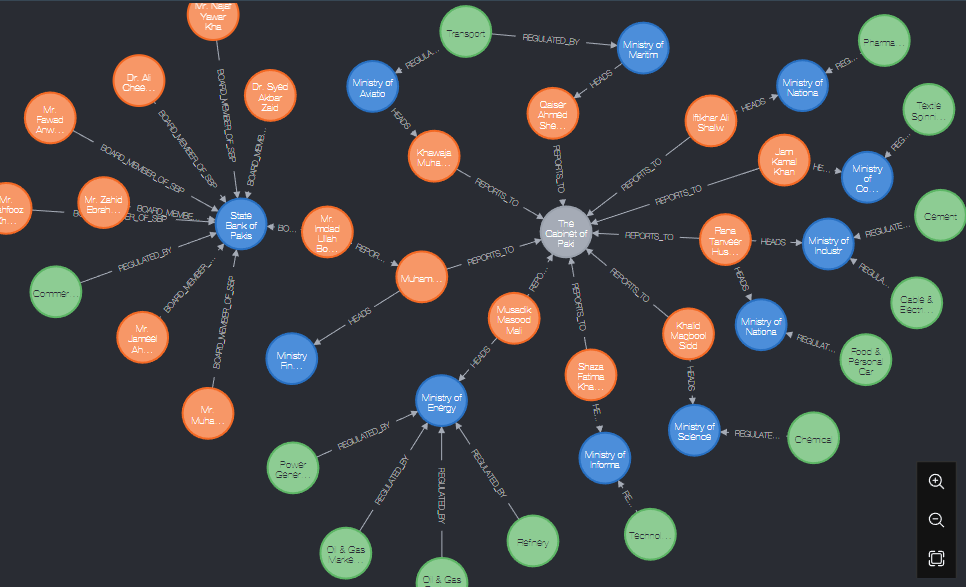
\includegraphics[width=0.9\textwidth]{Heirarchy.png} 
    \caption{Resultling Heirarchial Structure in Neo4j}
\end{figure}

\begin{figure}
    \centering
    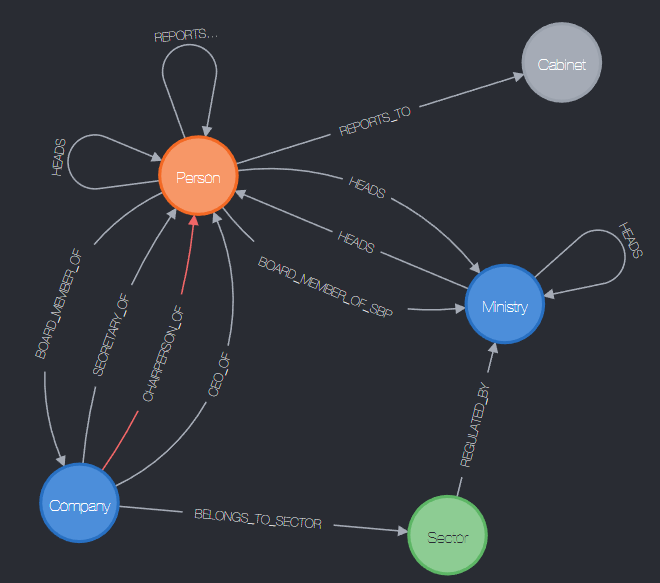
\includegraphics[width=0.8\textwidth]{Final_Model.png} 
    \caption{Final Model (CALL db.schema.visualization())}
\end{figure}

All in all, Our focus extends beyond mere financial metrics to explore the governance structures, regulatory frameworks, and inter-ministerial influences that shape the operational landscapes of these entities.
we aim to provide new insights into corporate governance and strategic alignments within Pakistan’s economic framework.


\section{Graph Analytics}
\subsection{Shortest Path}
\begin{lstlisting}[frame=single]
    MATCH (p1:Person {name: 'Dr. Salman Faridi'})
    MATCH (p2:Person {name: 'Mr. Saad Amanullah Khan'})
    return shortestPath((p1)-[*]-(p2))
\end{lstlisting}
\subsection{Centrality}
For this we will have to create our projection first!
\begin{lstlisting}[frame=single]
CALL gds.graph.project(
    'myGraph',  
    ['Person', 'Company', 'Ministry', 'Sector', 'Cabinet'],
    ['BOARD_MEMBER_OF', 'HEADS', 'BELONGS_TO_SECTOR', 'BOARD_MEMBER_OF_SBP', 'SECRETARY_OF', 'CHAIRPERSON_OF', 'REGULATED_BY', 'REPORTS_TO', 'CEO_OF']  
)
YIELD graphName, nodeCount, relationshipCount
RETURN graphName, nodeCount, relationshipCount
\end{lstlisting}
Next, we write querry for different types of centralities! That we will link to our Application:
\begin{lstlisting}[frame=single]
    CALL gds.degree.stream('myGraph')
    YIELD nodeId, score
    RETURN gds.util.asNode(nodeId).name AS name, score AS degree
    ORDER BY score DESC
    limit 30
\end{lstlisting}
Here is the projection for Betweenness Centrality. Relationship Orientation is Important here: Betweenness centrality frequently necessitates taking into account the path in both directions. UNDIRECTED specifies that the algorithm considers paths regardless of their directional flow.
\begin{lstlisting}[frame=single]
    CALL gds.graph.project(
        'boardMemberGraph',  // Name of the graph
        ['Person','Company', 'Ministry', 'Sector', 'Cabinet'],  // Node labels
        {
            BOARD_MEMBER_OF: {
                type: 'BOARD_MEMBER_OF',
                orientation: 'UNDIRECTED'
            },
            HEADS: {
                type: 'HEADS',
                orientation: 'UNDIRECTED'
            },
            SECRETARY_OF: {
                type: 'SECRETARY_OF',
                orientation: 'UNDIRECTED'
            },
            CHAIRPERSON_OF: {
                type: 'CHAIRPERSON_OF',
                orientation: 'UNDIRECTED'
            },
            REGULATED_BY: {
                type: 'REGULATED_BY',
                orientation: 'UNDIRECTED'
            },
            REPORTS_TO: {
                type: 'REPORTS_TO',
                orientation: 'UNDIRECTED'
            }
            // Include additional relationships as relevant
        }
    )
    YIELD graphName, nodeCount, relationshipCount
    RETURN graphName, nodeCount, relationshipCount
\end{lstlisting}

\begin{lstlisting}[frame=single]
    CALL gds.betweenness.stream('boardMemberGraph')
    YIELD nodeId, score
    RETURN gds.util.asNode(nodeId).name AS name, score AS betweenness
    ORDER BY score DESC
    LIMIT 20
\end{lstlisting}
One surprsing thing that resulted is was that Sui Southern Gas Company had higher score than The Cabinet of Pakistan. This means that the company lies more often on paths. This implies that when people are trying to connect with other people, Sui Southern Gas Company plays a more of pivotal role than Cabinet of Pakistan. I believe this is because they are perhaps easier to approach compared to the cabinet yet have as much influence over the corporate world. Either that or we can assume that they just have huge PR which allows them to connect with multiple companies, organisations and have events for instance.
\begin{figure}
    \centering
    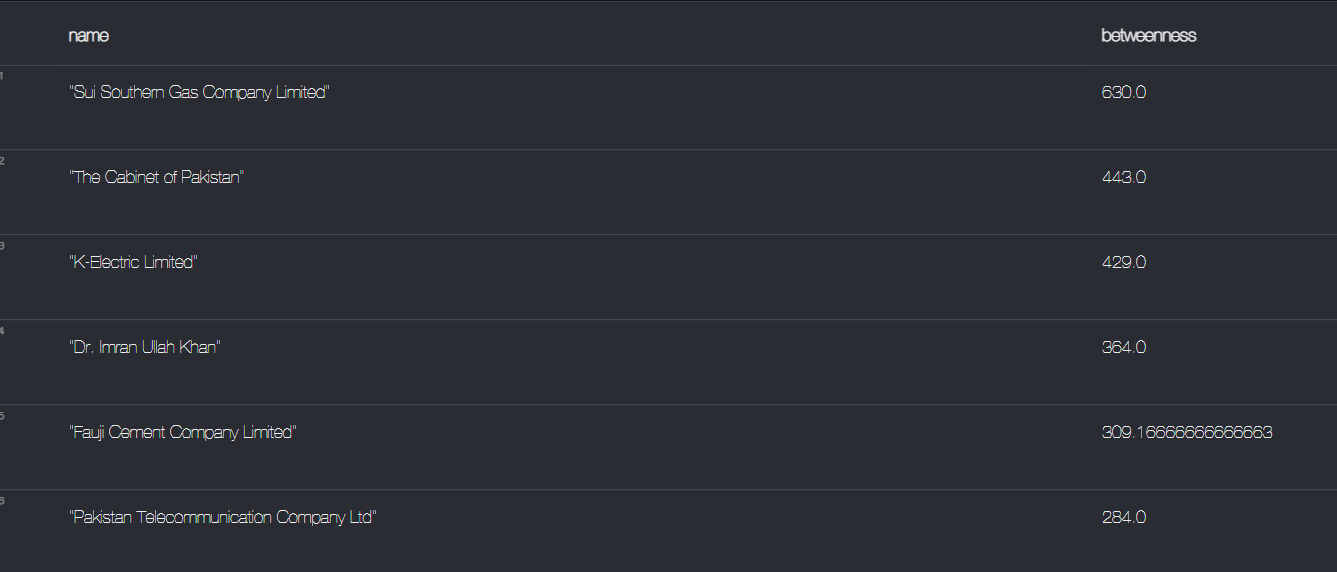
\includegraphics[width=0.9\textwidth]{betweenness.png} 
    \caption{Betweenness Centrality Results}
\end{figure}
\begin{lstlisting}[frame=single]
    CALL gds.graph.project(
    'closenessGraph',
    ['Person', 'Company'],
    {
        BOARD_MEMBER_OF: {
            type: 'BOARD_MEMBER_OF',
            orientation: 'UNDIRECTED'
        },
        CHAIRPERSON_OF: {
            type: 'CHAIRPERSON_OF',
            orientation: 'UNDIRECTED'
        },
        CEO_OF: {
            type: 'CEO_OF',
            orientation: 'UNDIRECTED'
        },
        SECRETARY_OF: {
            type: 'SECRETARY_OF',
            orientation: 'UNDIRECTED'
        }
    }
)
YIELD graphName, nodeCount, relationshipCount
RETURN graphName, nodeCount, relationshipCount

\end{lstlisting}
Now we look at Closeness Centrality, this time we have restricted it to Person and Company Nodes.   
\begin{lstlisting}[frame=single]
    CALL gds.closeness.stream('closenessGraph')
    YIELD nodeId, score
    RETURN gds.util.asNode(nodeId).name AS name, score AS closeness
    ORDER BY closeness DESC
    LIMIT 30
\end{lstlisting}
The results are fairly standard and almost all companies had score of 1.0. Person had lower than that. \\
Lastly, we look at PageRank Complexity:
\begin{lstlisting}[frame=single]
    CALL gds.graph.project(
        'pageRankGraph',
        ['Person', 'Company', 'Ministry', 'Sector'],
        {
            BOARD_MEMBER_OF: {
                type: 'BOARD_MEMBER_OF',
                orientation: 'NATURAL'
            },
            HEADS: {
                type: 'HEADS',
                orientation: 'NATURAL'
            },
            REGULATED_BY: {
                type: 'REGULATED_BY',
                orientation: 'REVERSE'
            },
            CEO_OF: {
                type: 'CEO_OF',
                orientation: 'NATURAL'
            }
        }
    )
    YIELD graphName, nodeCount, relationshipCount
    RETURN graphName, nodeCount, relationshipCount    
\end{lstlisting}
\begin{lstlisting}[frame=single]
    CALL gds.pageRank.stream('pageRankGraph')
    YIELD nodeId, score
    RETURN gds.util.asNode(nodeId).name AS name, score AS pageRank
    ORDER BY score DESC
    LIMIT 20
\end{lstlisting}
(NEXT PAGE)\\
We got different results this time, likely due to the High PageRank nodes being nearer to the important ones. This proves that PageRank considers the global context and does not rely solely on shortest path and its derivatives.
However, this seems irrelavant in the context of this network. We can also think about this in this way that since they are near Ifluential nodes, they are likely to become influential in the future.
For the currently influential nodes (Company/People), knowing which entities are viewed as influential by them and their peers (as highlighted by PageRank) versus being central by structure themselves (as shown by betweenness or closeness), they can do strategic planning accordingly.
\begin{figure}
    \centering
    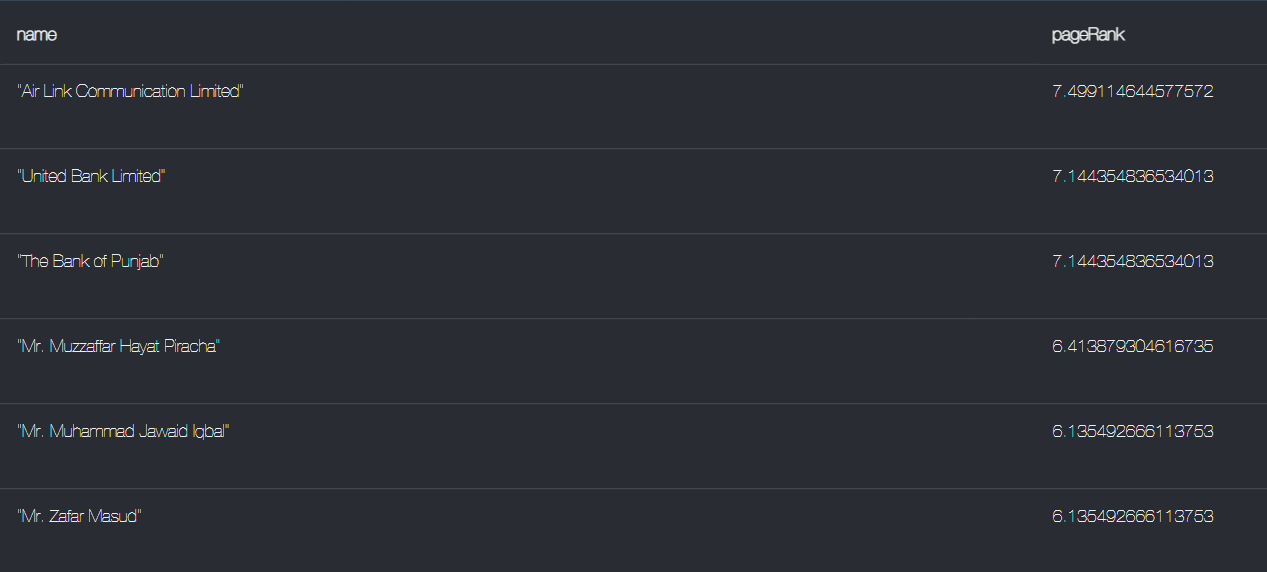
\includegraphics[width=0.9\textwidth]{pagerank.png} 
    \caption{PageRank Results}
\end{figure}
\section{Adding Features}
\begin{lstlisting}[frame=single]
    CALL gds.graph.project(
    'unifiedGraph',
    ['Person', 'Company', 'Ministry', 'Sector', 'Cabinet'],
    {
        BOARD_MEMBER_OF: {type: 'BOARD_MEMBER_OF', orientation: 'UNDIRECTED'},
        HEADS: {type: 'HEADS', orientation: 'UNDIRECTED'},
        REGULATED_BY: {type: 'REGULATED_BY', orientation: 'UNDIRECTED'},
        CEO_OF: {type: 'CEO_OF', orientation: 'UNDIRECTED'},
        REPORTS_TO: {type: 'REPORTS_TO', orientation: 'UNDIRECTED'},
        CHAIRPERSON_OF: {type: 'CHAIRPERSON_OF', orientation: 'UNDIRECTED'},
        SECRETARY_OF: {type: 'SECRETARY_OF', orientation: 'UNDIRECTED'},
        BELONGS_TO_SECTOR: {type: 'BELONGS_TO_SECTOR', orientation: 'UNDIRECTED'}
    }
)
YIELD graphName, nodeCount, relationshipCount
RETURN graphName, nodeCount, relationshipCount
\end{lstlisting}
\begin{lstlisting}[frame=single]
    CALL gds.pageRank.write('unifiedGraph', {
        writeProperty: 'pageRank'
    });
    CALL gds.betweenness.write('unifiedGraph', {
        writeProperty: 'betweenness'
    });
    CALL gds.closeness.write('unifiedGraph', {
        writeProperty: 'closeness'
    });
    CALL gds.degree.write('unifiedGraph', {
        writeProperty: 'degree'
    });
\end{lstlisting}
\begin{lstlisting}[frame=single]
    CALL gds.beta.pipeline.linkPrediction.create('linkPredictionPipeline')
\end{lstlisting}
\pagebreak
\section{Tkinter Front End}
Using Python's Library, Tkinter we designed a simple user-interface, where all of the above-mentioned section's querries are run with a click of a button. We used py2neo library to load our graph database (Password: 12345678).
\begin{figure}[H]
    \centering
    \includegraphics[width=0.8\textwidth]{frontend.png} 
    \caption{Tkinter-based Front End Design}
\end{figure}
\pagebreak
\section{References}
\begin{enumerate}
    \item Pakistan Stock Exchange. \url{https://www.psx.com.pk/}
    \item Cabinet of Pakistan. \url{https://en.wikipedia.org/wiki/Cabinet_of_Pakistan}
    \item Ministry of Foreign Affairs, Government of Pakistan. \url{https://na.gov.pk/en/fmins_list.php}
\end{enumerate}

\end{document}
